\documentclass[a4paper, 10pt, notitlepage]{article}
\usepackage[english]{babel}
\usepackage[latin1]{inputenc}
\usepackage{amsmath}
\usepackage{amsfonts}
\usepackage{graphicx}
\usepackage{url}
\usepackage{layaureo}
\author{G. Bertoli \and A. Shcherbakova \and E. Valdes}
\title{Measurements of Current - Voltage and Capacitance - Voltage curves for
  irradiated and non irradiated silicon detectors}
\date{2 November 2015}
\graphicspath{{/home/drkg4b/work/detector_school/lab_reports/images/}}
\begin{document}
\maketitle

\section{Introduction}
\label{sec:intro}

Current-Voltage (IV) and Capacitance-Voltage(CV) curves are used to charaterize
silicon dectectors. In particular, the IV curve is used to determine the leakage
current value and the CV curve to measure the depletion voltage. The results
from these measurements can be used to determine aging and radiation damage, for
quality control and comparison of different manufacturing methods. The IV and CV
curves of three different diodes, p-type passivated, n-type and n-type
irradiated were measured and the quality of the latter checked.

\begin{figure}[!h]
  \centering
  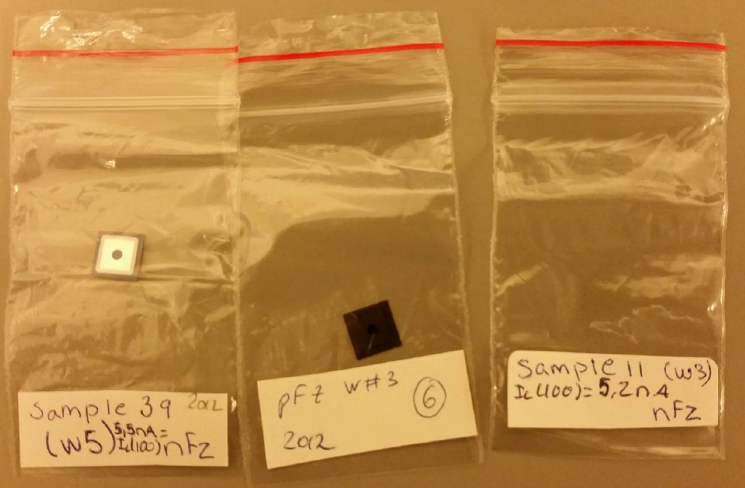
\includegraphics[width=.5\linewidth]{three_diodes}
    \caption{The three tested samples.}
  \label{fig:three_diodes}
\end{figure}
\section{Setup and measurements}
\label{sec:setup}

The CV-IV probe station used consists of a PC with custom LabView based software
(CIVility) for control and data acquisition, a platform with probe needles, a
light source, a microscope, a cable connection pad, a vacuum pump and a dark
box. The probe station measuring devices are a source meter unit, a picoamper
meter and a capacitance meter.

To perform the measurement the diodes were positioned on the platform below the
microscope and the left probe needle was connected to the guard ring while the
right one was connected to the square contact pad to provide a reverse bias
voltage.

Two configurations were used for each sample, one to measure the IV curve and
the other one for the CV curve, this part was handled by the assistant. The dark
box was then closed and the data acquisition system started. The capacitance and
the current were measured in steps of 5 volts from 0 to 350 V, this reverse bias
will attract charge carriers away from the junction increasing the depletion
reagion.
\end{document}
%%% Local Variables:
%%% mode: latex
%%% TeX-master: t
%%% End:
